在我们讨论Clang中的编译器驱动程序之前,有必要强调一下:编译一段代码绝不是单一的任务(也不是简单的任务)。学校里,老师们教导我们,编译器包括一个\textbf{词法分析器},一个\textbf{解析器},有时附带一个\textbf{优化器},最后是一个\textbf{汇编代码打印器}。虽然在实际编译器中仍然可以看到这些阶段,但它们提供的只是文本汇编代码,而不是期望的可执行文件或库。此外,这个原生编译器的灵活性非常有限——不能移植到任何其他操作系统或平台上。

为了让这个玩具编译器更真实和可用,许多其他管道工工具需要放在一起,以及核心编译器:一个将汇编代码转换为(二进制格式)对象文件的\textbf{汇编器},一个将多个对象文件放入可执行文件或库的\textbf{链接器},以及许多其他解析平台特定配置的例程,如:数据宽度、默认头文件路径或\textbf{应用二进制接口(ABIs)}。只有在这些“水管工”的帮助下,我们才能通过输入几个单词来使用编译器:

\begin{tcblisting}{commandshell={}}
$ clang hello_world.c -o hello_world
\end{tcblisting}

编译器驱动是组织这些“管道工”工作的软件。尽管在编译过程中有多个不同的任务要做,本章中我们只关注两个最重要的任务——处理编译器标志和在不同平台上调用正确的工具——这就是工具链的设计目的。

下图显示了驱动、工具链和编译器其余部分之间的交互信息:

\hspace*{\fill} \\ %插入空行
\begin{center}
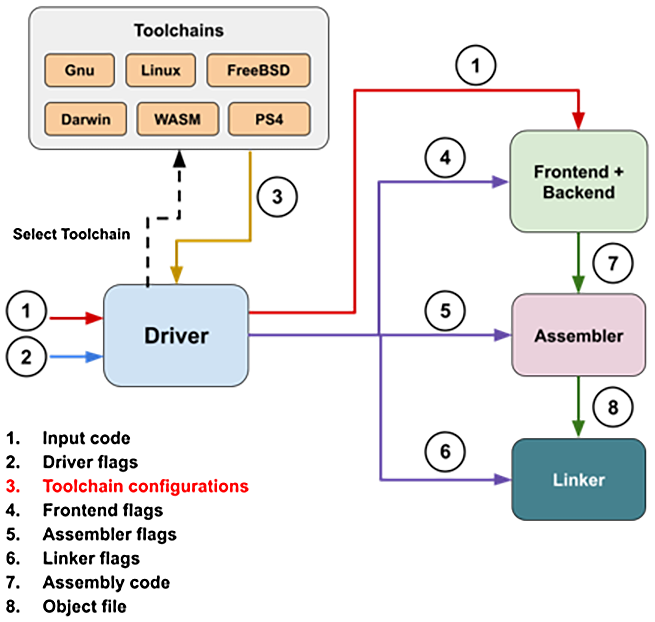
\includegraphics[width=0.8\textwidth]{content/2/chapter8/images/1.png}\\
图8.1 - Clang的驱动程序、工具链和其他编译器的常规工作流程
\end{center}

如上图所示,Clang的驱动充当了\textit{调度器},将标志和工作负载分配到每个编译阶段,即前端/后端、汇编器和链接器。为了更具体地了解每个阶段的标志是什么样子,回想一下在本章开始时介绍的\texttt{-\#\#\#}编译器选项。该选项打印的(大量)内容是前端的标志(上图中为4),例如:在这些前端标志中,\texttt{-internal-system}携带关于系统头文件路径的信息,包括C/C++标准库头文件存储的路径。很明显,Clang的前端需要知道标准库的头文件存储在哪里,但根据使用\texttt{clang}(或\texttt{gcc})的经验,使用者很少需要明确地告诉它们这些头文件存储在哪里——因为驱动来做这件事。同样的逻辑也适用于链接阶段。连接器通常需要不仅需要一个目标文件来正确地生成可执行文件或库,例如:需要知道C/C++标准库的库文件位置(比如在Unix/Linux系统上的\texttt{*.a}或\texttt{*.so})。在这种情况下,Clang的驱动将通过链接器标志向链接器提供该信息。

提供给各个编译器阶段的标志和工作负载——简而言之,就是\textit{配置}——从两个来源转换而来:驱动标志(上图中有2个)和所选的工具链(上图中有3个)。驱动标志是由用户通过命令行界面提供的——也就是编译器标志——例如:\texttt{-c},\texttt{-Wall}和\texttt{-std=c++11}。下一节中,我们将展示一些Clang如何将驱动标志转换为前端标志,甚至汇编器/链接器标志的示例。

另外,\textbf{工具链}是描述应该如何在特定平台上编译输入代码的实体。不同的硬件体系结构和操作系统(OS)——简称平台——有自己的构建、加载和运行程序的方式。以macOS X和Linux为例,虽然它们都有一个类unix的环境,但当构建一个程序时,macOS X的系统(标准)库总是在Apple的XCode IDE包中,而Linux通常将它们存储在普通的文件夹中,如\texttt{/usr/include}和\texttt{/usr/lib}。此外,macOS X使用一种称为\textbf{Mach-O}的可执行格式,与于Linux的ELF格式不同。这极大地影响了编译器(Clang)构建代码的方式。

Clang要为不同的平台编译代码,使用工具链(内部由\texttt{ToolChain} C++类表示)来封装特定于平台的信息和配置。编译的早期阶段,Clang的驱动会根据当前运行的系统(主机系统)或者用户的偏好选择一个正确的工具链——可以使用\texttt{-target=}驱动标志来要求Clang为不同于主机系统的特定平台构建一个程序,这是有效的\textbf{交叉编译}。然后,驱动将从选择的工具链中收集一些特定于平台的配置,然后将其与前面提到的驱动程序选项结合起来,并通过命令行标志将它们分派到各个编译器阶段。请注意,不同的平台通常使用不同的汇编器和连接器,例如:macOS X目前只能使用\texttt{ld64}和\texttt{lld}连接器,而Linux可以使用\texttt{ld}(BFD连接器)、\texttt{ld.gold}和\texttt{lld}作为连接器。因此,工具链还应该指定使用什么汇编器和链接器。本章的最后一节,添加一个自定义工具链,我们将通过一个示例项目来学习Clang的工具链是如何工作的。让我们开始旅程,如何在Clang的驱动标示是如何工作的。






























